\chapter{Tecnologias e Plataformas de IoT}

\section{Novos Protocolos}
\subsection{6LoWPAN}
Possui como objetivo principal possibilitar a comunica\c{c}\~ao atrav\'es do protocolo IPv6 nas redes PAN(IEEE 802.15.4), definida para cria\c{c}\~ao de redes sem fio pessoais com baixo consumo de energia e habilitando a conex\~ao \`a internet de micro componentes e sensores. Esse protocolo se apoia na concep\c{c}\~ao de que a Internet \'e integralmente constru\'ida com IPs e cada dispositivo conectado possui seu pr\'oprio IP o tornando parte de um todo no mundo da Internet ou melhor na Internet das Coisas.
\subsection{RPL}
De forma um pouco diferente ao 6LoWPAN, esse protocolo focou em atender \`a diversidade de requisitos e aplica\c{c}\~oes presentes no mundo da Internet das Coisas. Vai desde a sua utiliza\c{c}\~ao nas redes urbanas (smart cities), passando pela automatiza\c{c}\~ao de casas e edif\'icios(smart homes and buildings) at\'e o suporte \`a outros tipos de automatiza\c{c}\~ao (smart spaces, smart cars, etc). Para atingir seu objetivo ele usa como base a teoria dos grafos ac\'iclicos direcionados (do ingl\^es DAG) para criar sua topologia, viabilizando a utiliza\c{c}\~ao de um protocolo de roteamento para cria\c{c}\~ao de suas pr\'oprias rotas contendo um ou mais destinos orientados que s\~ao atualizados em intervalos aleat\'orios de tempo.
\subsection{CoAP}
Protocolo de transmiss\~ao web desenhado espec\'ificamente para uso em aplica\c{c}\~oes M2M (machine-to-machine) como smart energy e smart homes, onde suas redes e n\'os ficam restritos dentro de seu pr\'oprio ecossistema. Ele foi desenhado para utilizar uma quantidade m\'inima de recursos do dispositivo e da rede, utilizando o j\'a consolidado UDP no lugar de construir uma pilha de transporte complexa. Na linha de seguran\c{c}a o CoAP prop\~oe par\^ametros DTLS equivalentes \`as chaves RSA de 3072 bits, conseguindo manter um n\'ivel aceit\'avel de performance at\'e nos menores n\'os.
\subsection{Dash7}
Protocolo de redes sem fio de c\'odigo aberto criado para uso especifico em sensores e atuadores que operam nas bandas n\~ao licenciadas das frequ\^encias 433MHz, 868MHz e 915MHz. Assim como o 6LoWPAN, ele foi idealizado para uso em equipamentos com baixo consumo de energia, por\'em seus criadores se preocuparam na constru\c{c}\~ao de um protocolo completo, que dispusesse de longo alcance (at\'e 2 km), tivesse uma lat\^encia de conex\~ao reduzida nos dispositivos em movimento, fosse uma pilha de protocolos pequena, suportasse chaves de criptografia AES com 128-bit, atingindo taxas de transfer\^encia de dados adequadas aos dispositivos de IoT (at\'e  167 kbit/s).
\subsection{MQTT}

\section{Plataformas}
\subsection{Thingspeak}
	Plataforma Web open-sourse seguindo a linha da "Web das Coisas", onde "coisas" se conectam \`a APIs remotas utilizando a internet e seus protocolos. Ele funciona de forma semelhante a um Middleware baseado na nuvem onde end-points s\~ao criados para serem utilizados por webnodes (n\'os de sensores) para remeter solicita\c{c}\~oes, enviar dados para serem armazenados e solicitar a recupera\c{c}\~ao de informa\c{c}\~oes utilizando o protocolo HTTP via Internet. O foco principal do Thingspeak \'e utilizar aplicar as seguintes atividades de minera\c{c}\~ao de dados na Internet das Coisas:
	
	\begin{itemize}
		\item Coleta - Enviar dados dos sensores para a nuvem.
		\item An\'alise - Analisar e Visualizar informa\c{c}\~oes com MATLAB.
		\item A\c{c}\~ao - Reagir a uma informa\c{c}\~ao acionando uma a\c{c}\~ao
	\end{itemize}
	
	Com o Thingspeak(Figura~\ref{fig:arqthings}) o usu\'ario poder\'a criar remotamente funcionalidades para monitoramento de seus sensores Ub\'iquos ("coisas") conectados em sua rede, rastreamento dos objetos conectados e tamb\'em criar uma rede social de coisas (monitorando atualiza\c{c}\~oes de status). Por\'em, mais que apenas criar APIs de monitoramento remoto dos dados, o Thingspeak de forma integrada o uso do MATLAB (aplica\c{c}\~ao de alta performance voltada para c\'alculo num\'erico) para an\'alise, tratamento dos dados coletados com base em regras pr\'e-definidas pelo usu\'ario para agrega\c{c}\~ao dos dados e tomada de decis\~ao, visualizando seus informa\c{c}\~oes de forma refinada em seu dashboard.
	
	
	\begin{figure}[ht]
		\centering
		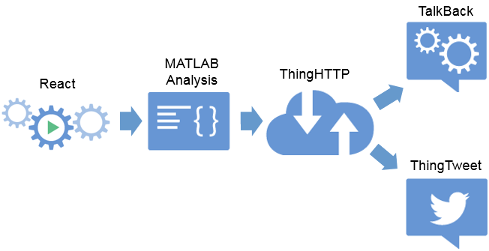
\includegraphics[width=.5\textwidth]{fig8.png}
		\caption{Exemplo de uso do Thingspeak}
		\label{fig:arqthings}
	\end{figure}
	
	
	Para iniciar um prot\'otipo na ferramenta~\cite{KRISHNA2014}, \'e necess\'ario uma das seguintes placas de prototipagem: Arduino(com shield de Ethernet ou Wi-Fi), Particle Core/Photon/Electron, Raspberry PI ou Electric Imp; conectadas \`a Internet e configurados com a biblioteca pr\'opria do Thingspeak que far\'a a comunica\c{c}\~ao com os servidores remotos atrav\'es de opera\c{c}\~oes GET e POST do protocolo HTTP.
	
	Ao configurar dispositivos para conectar ao ThingSpeak, os usu\'arios ter\~ao dispon\'iveis as seguintes funcionalidades para trabalhar:
	\begin{labeling}{Event scheduling}
		\item[Data collection] Criar novos canais para coleta dos dados que ser\~ao analizados.
		\item[Open API] APIs REST dispon\'iveis para gest\~ao e publica\c{c}\~ao remota de feeds, canais e a\c{c}\~oes.
		\item[Alerts] Apps dispon\'iveis para monitorar e notificar ocorr\^encia de eventos.
		\item[Event scheduling] App para controle de acionamento de a\c{c}\~oes com base em regras temporais pr\'e-definidas.
		\item[MATLAB] ()analytics and visualizations) App para an\'alise de dados e elimina\c{c}\~ao de "Outliers" em um canal usando fun\c{c}\~oes do MatLab.
		\item[MQTT] (publish support)APIs MQTT dispon\'iveis para publica\c{c}\~ao de mensagens nos Feeds pelo broker MQTT.
		\item[App integrations] Integrar canais de coleta aos apps de transforma\c{c}\~ao dos dados, acionamento de a\c{c}\~oes e visualiza\c{c}\~ao.
	\end{labeling}
	
	O Thingspeak integrado aos recursos do MatLab se mostra uma ferramenta muito adequada para criar fluxos de notifica\c{c}\~ao e controle automatizado a partir da minera\c{c}\~ao dos dados provenientes de uma rede de sensores conectados \`a Web que exija c\'alculos matem\'aticos no processamento, mantendo um alto rendimento. H\'a ainda a possibilidade de utiliza\c{c}\~ao dos recursos de processamento e a\c{c}\~ao do Thingspeak, para cria\c{c}\~ao de regras de intelig\^encia computacional para uso em projetos voltados \`a Intelig\^encia Ambiental, Intelig\^encia Artificial e SWoT. 

%\subsection{instructables}
%\subsection{code project}
%\subsection{channel9}

\subsection{Pachube/Xively}
	Inicialmente criada com o objetivo de se tornar uma rede social para a Internet das Coisas, dando suporte para comunidades virtuais criarem uma infraestrutura de dados compartilhados, foi adquirida pela empresa LogMeIn em 2011, passando a ser um servi\c{c}o de plataforma para a Internet das Coisas, com objetivo de disponibilizar uma plataforma onde voc\^e pode criar produtos conectados que s\~ao operados (Figura~\ref{fig:arqxively}), controlados e automatizados de forma simples utilizando a internet e viabilizando a identifica\c{c}\~ao de insights dos usu\'arios a partir da an\'alise dos dados.
	
	\begin{figure}[ht]
		\centering
		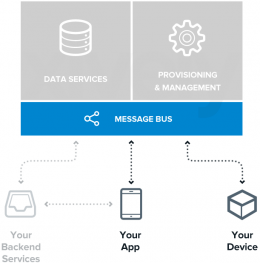
\includegraphics[width=.5\textwidth]{fig7.png}
		\caption{Arquitetura do Xively}
		\label{fig:arqxively}
	\end{figure}
	
	
	Segundo o site da plataforma ~\cite{XIVELY} esses s\~ao os 7 elementos para se criar um produto conectado na Internet das Coisas:
	
	\begin{itemize}
		\item Conceitualizar e definir produto conectado
		\item Fazer prova de conceito com hardware (Seguran\c{c}a)
		\item Desenvolver apps onde usu\'arios podem monitorar seu dispositivo
		\item Habilitar plataforma onde empresa inclui e gerencia seus dispositivos conectados
		\item Integrar dados de dispositivo com ferramenta de relacionamento com clientes 
		\item Preparar ferramenta de an\'alise dos dados para obter insight de usu\'arios
		\item Criar novos canais de engajamento dos usu\'arios ao produto
	\end{itemize}
	
	Alguns exemplos de produtos conectados na plataforma seriam: 
	\begin{labeling}{M\'aquina de lavar}
		\item[M\'aquina de lavar] Identificaria a ocorrencia de algum problema, solicite as pe\c{c}as v\~ao precisar reparo na f\'abrica, chame o t\'ecnico informando a falha identificada e notifique o dono sobre a falha e quanto vai custar o conserto. 
		\item[Carro] Identificaria a hora de uma revis\~ao, verifique a agenda do cliente e cruze com as datas dispon\'iveis na concession\'aria, agendando o melhor hor\'ario, informando a manuten\c{c}\~ao necess\'aria e o custo.
	\end{labeling}

\subsection{IFTTT}
	A concep\c{c}\~ao essencial dessa plataforma \'e automatizar "coisas" utilizando condi\c{c}\~oes(Figura~\ref{fig:ifttt}), assim como o significado de seu acr\^onimo diz: "Se acontecer isso, ent\~ao fa\c{c}a aquilo" (If This, Then That). Ele \'e tanto um website como um app mobile lan\c{c}ado em 2010 com o slogan "Coloque a internet para trabalhar para voc\^e" e com objetivo de automatizar tudo o que for poss\'ivel, desde tarefas nos seus apps e sites favoritos at\'e gadgets e dispositivos inteligentes. A plataforma possui 4 elementos.
	
	\begin{labeling}{Receitas/Applets}
		\item[Gatilhos] "Se" da condi\c{c}\~ao desejada
		\item[A\c{c}\~oes] "Aquilo" da condi\c{c}\~ao desejada
		\item[Receitas/Applets] Condi\c{c}\~oes, ou uni\~ao de um trigger com uma action
		\item[Canais/Servi\c{c}os]  Descri\c{c}\~ao dos dados de um certo servi\c{c}o
	\end{labeling}
	
	Atualmente a plataforma suporta mais de 110 servi\c{c}os ("canais") incluindo apps para dispositivos Android e Apple iOS como Lembretes e Fotos, e tamb\'em sites web como Facebook, Instagram, Flickr, Tumblr, Google Calendar, Google Drive, Feedly, Foursquare, LinkedIn, SoundCloud, WordPress, YouTube, e muitos outros.
	
	\begin{figure}[ht]
		\centering
		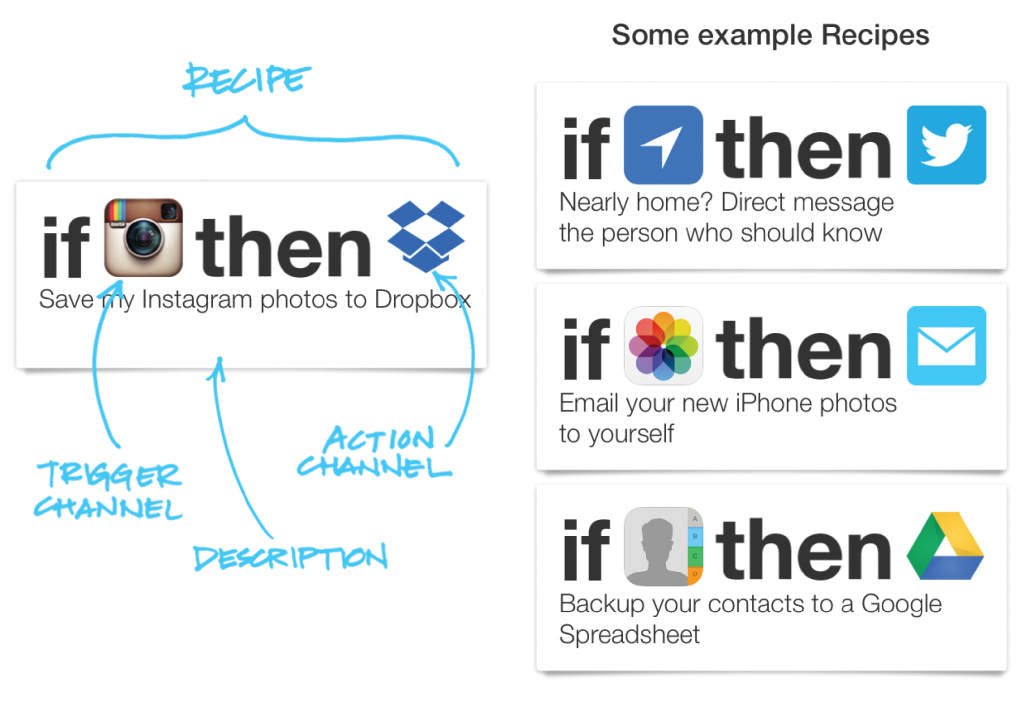
\includegraphics[width=.5\textwidth]{fig5.png}
		\caption{Exemplo de automatiza\c{c}\~ao no IFTTT}
		\label{fig:ifttt}
	\end{figure}
	
	diminuir a sua perda de tempo, automatizandos todas as "coisas" poss\'iveis e criando canais onde voc\^e possa verificar as informa\c{c}\~oes que precisa.  com tantas "coisas" virtuais no mundo querendo tomar a sua aten\c{c}\~ao, porqu\^e n\~ao automatizar tudo o que for poss\'ivel e caso seja realmente necess\'ario a sua aten\c{c}\~ao, voc\^e seja 
	
